% Created by tikzDevice version 0.12.6 on 2026-07-09 15:42:24
% !TEX encoding = UTF-8 Unicode
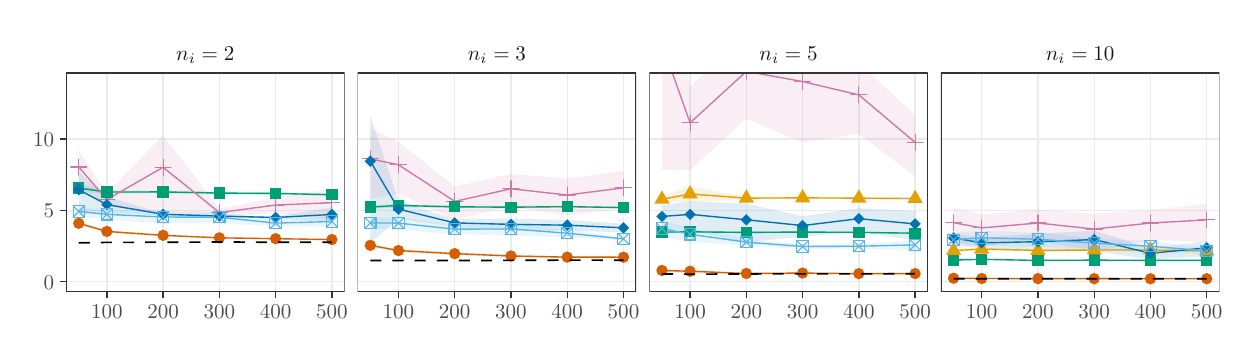
\begin{tikzpicture}[x=1pt,y=1pt]
\definecolor{fillColor}{RGB}{255,255,255}
\path[use as bounding box,fill=fillColor,fill opacity=0.00] (0,0) rectangle (433.62,108.41);
\begin{scope}
\path[clip] (  0.00,  0.00) rectangle (433.62,108.41);
\definecolor{drawColor}{RGB}{255,255,255}
\definecolor{fillColor}{RGB}{255,255,255}

\path[draw=drawColor,line width= 0.5pt,line join=round,line cap=round,fill=fillColor] ( -0.00,  0.00) rectangle (433.62,108.41);
\end{scope}
\begin{scope}
\path[clip] ( 13.87, 12.99) rectangle (114.50, 92.09);
\definecolor{fillColor}{RGB}{255,255,255}

\path[fill=fillColor] ( 13.87, 12.99) rectangle (114.50, 92.09);
\definecolor{drawColor}{gray}{0.92}

\path[draw=drawColor,line width= 0.5pt,line join=round] ( 13.87, 16.58) --
	(114.50, 16.58);

\path[draw=drawColor,line width= 0.5pt,line join=round] ( 13.87, 42.38) --
	(114.50, 42.38);

\path[draw=drawColor,line width= 0.5pt,line join=round] ( 13.87, 68.18) --
	(114.50, 68.18);

\path[draw=drawColor,line width= 0.5pt,line join=round] ( 28.61, 12.99) --
	( 28.61, 92.09);

\path[draw=drawColor,line width= 0.5pt,line join=round] ( 48.94, 12.99) --
	( 48.94, 92.09);

\path[draw=drawColor,line width= 0.5pt,line join=round] ( 69.27, 12.99) --
	( 69.27, 92.09);

\path[draw=drawColor,line width= 0.5pt,line join=round] ( 89.60, 12.99) --
	( 89.60, 92.09);

\path[draw=drawColor,line width= 0.5pt,line join=round] (109.92, 12.99) --
	(109.92, 92.09);
\definecolor{fillColor}{RGB}{213,94,0}

\path[fill=fillColor,fill opacity=0.12] ( 18.45, 38.32) --
	( 28.61, 35.20) --
	( 48.94, 33.63) --
	( 69.27, 32.68) --
	( 89.60, 32.36) --
	(109.92, 31.98) --
	(109.92, 31.70) --
	( 89.60, 31.97) --
	( 69.27, 32.27) --
	( 48.94, 33.07) --
	( 28.61, 34.35) --
	( 18.45, 37.09) --
	cycle;

\path[] ( 18.45, 38.32) --
	( 28.61, 35.20) --
	( 48.94, 33.63) --
	( 69.27, 32.68) --
	( 89.60, 32.36) --
	(109.92, 31.98);

\path[] (109.92, 31.70) --
	( 89.60, 31.97) --
	( 69.27, 32.27) --
	( 48.94, 33.07) --
	( 28.61, 34.35) --
	( 18.45, 37.09);
\definecolor{fillColor}{RGB}{0,158,115}

\path[fill=fillColor,fill opacity=0.12] ( 18.45, 51.86) --
	( 28.61, 49.65) --
	( 48.94, 49.53) --
	( 69.27, 49.20) --
	( 89.60, 48.94) --
	(109.92, 48.52) --
	(109.92, 47.56) --
	( 89.60, 48.08) --
	( 69.27, 48.06) --
	( 48.94, 48.58) --
	( 28.61, 48.38) --
	( 18.45, 48.99) --
	cycle;

\path[] ( 18.45, 51.86) --
	( 28.61, 49.65) --
	( 48.94, 49.53) --
	( 69.27, 49.20) --
	( 89.60, 48.94) --
	(109.92, 48.52);

\path[] (109.92, 47.56) --
	( 89.60, 48.08) --
	( 69.27, 48.06) --
	( 48.94, 48.58) --
	( 28.61, 48.38) --
	( 18.45, 48.99);
\definecolor{fillColor}{RGB}{0,114,178}

\path[fill=fillColor,fill opacity=0.12] ( 18.45, 56.50) --
	( 28.61, 47.26) --
	( 48.94, 41.34) --
	( 69.27, 40.60) --
	( 89.60, 40.16) --
	(109.92, 43.44) --
	(109.92, 38.08) --
	( 89.60, 39.48) --
	( 69.27, 40.06) --
	( 48.94, 40.58) --
	( 28.61, 41.40) --
	( 18.45, 41.56) --
	cycle;

\path[] ( 18.45, 56.50) --
	( 28.61, 47.26) --
	( 48.94, 41.34) --
	( 69.27, 40.60) --
	( 89.60, 40.16) --
	(109.92, 43.44);

\path[] (109.92, 38.08) --
	( 89.60, 39.48) --
	( 69.27, 40.06) --
	( 48.94, 40.58) --
	( 28.61, 41.40) --
	( 18.45, 41.56);
\definecolor{fillColor}{RGB}{204,121,167}

\path[fill=fillColor,fill opacity=0.12] ( 18.45, 64.01) --
	( 28.61, 48.53) --
	( 48.94, 69.53) --
	( 69.27, 43.00) --
	( 89.60, 46.97) --
	(109.92, 50.19) --
	(109.92, 39.04) --
	( 89.60, 41.35) --
	( 69.27, 40.12) --
	( 48.94, 41.46) --
	( 28.61, 43.90) --
	( 18.45, 51.15) --
	cycle;

\path[] ( 18.45, 64.01) --
	( 28.61, 48.53) --
	( 48.94, 69.53) --
	( 69.27, 43.00) --
	( 89.60, 46.97) --
	(109.92, 50.19);

\path[] (109.92, 39.04) --
	( 89.60, 41.35) --
	( 69.27, 40.12) --
	( 48.94, 41.46) --
	( 28.61, 43.90) --
	( 18.45, 51.15);
\definecolor{fillColor}{RGB}{86,180,233}

\path[fill=fillColor,fill opacity=0.12] ( 18.45, 43.47) --
	( 28.61, 42.77) --
	( 48.94, 42.01) --
	( 69.27, 41.88) --
	( 89.60, 38.91) --
	(109.92, 40.08) --
	(109.92, 36.50) --
	( 89.60, 36.60) --
	( 69.27, 37.78) --
	( 48.94, 37.77) --
	( 28.61, 38.98) --
	( 18.45, 40.40) --
	cycle;

\path[] ( 18.45, 43.47) --
	( 28.61, 42.77) --
	( 48.94, 42.01) --
	( 69.27, 41.88) --
	( 89.60, 38.91) --
	(109.92, 40.08);

\path[] (109.92, 36.50) --
	( 89.60, 36.60) --
	( 69.27, 37.78) --
	( 48.94, 37.77) --
	( 28.61, 38.98) --
	( 18.45, 40.40);
\definecolor{drawColor}{RGB}{213,94,0}

\path[draw=drawColor,line width= 0.5pt,line join=round] ( 18.45, 37.71) --
	( 28.61, 34.78) --
	( 48.94, 33.36) --
	( 69.27, 32.47) --
	( 89.60, 32.16) --
	(109.92, 31.84);
\definecolor{drawColor}{RGB}{0,158,115}

\path[draw=drawColor,line width= 0.5pt,line join=round] ( 18.45, 50.45) --
	( 28.61, 49.02) --
	( 48.94, 49.06) --
	( 69.27, 48.64) --
	( 89.60, 48.51) --
	(109.92, 48.04);
\definecolor{drawColor}{RGB}{0,114,178}

\path[draw=drawColor,line width= 0.5pt,line join=round] ( 18.45, 49.88) --
	( 28.61, 44.48) --
	( 48.94, 40.97) --
	( 69.27, 40.33) --
	( 89.60, 39.82) --
	(109.92, 40.91);
\definecolor{drawColor}{RGB}{204,121,167}

\path[draw=drawColor,line width= 0.5pt,line join=round] ( 18.45, 58.08) --
	( 28.61, 46.30) --
	( 48.94, 57.95) --
	( 69.27, 41.60) --
	( 89.60, 44.31) --
	(109.92, 45.16);
\definecolor{drawColor}{RGB}{86,180,233}

\path[draw=drawColor,line width= 0.5pt,line join=round] ( 18.45, 41.98) --
	( 28.61, 40.95) --
	( 48.94, 39.99) --
	( 69.27, 39.92) --
	( 89.60, 37.79) --
	(109.92, 38.36);
\definecolor{fillColor}{RGB}{213,94,0}

\path[fill=fillColor] ( 18.45, 37.71) circle (  2.05);
\definecolor{drawColor}{RGB}{204,121,167}

\path[draw=drawColor,line width= 0.4pt,line join=round,line cap=round] ( 15.55, 58.08) -- ( 21.35, 58.08);

\path[draw=drawColor,line width= 0.4pt,line join=round,line cap=round] ( 18.45, 55.18) -- ( 18.45, 60.98);
\definecolor{fillColor}{RGB}{0,158,115}

\path[fill=fillColor] ( 16.40, 48.40) --
	( 20.50, 48.40) --
	( 20.50, 52.51) --
	( 16.40, 52.51) --
	cycle;
\definecolor{fillColor}{RGB}{0,114,178}

\path[fill=fillColor] ( 16.40, 49.88) --
	( 18.45, 51.93) --
	( 20.50, 49.88) --
	( 18.45, 47.82) --
	cycle;
\definecolor{drawColor}{RGB}{86,180,233}

\path[draw=drawColor,line width= 0.4pt,line join=round,line cap=round] ( 16.40, 39.93) rectangle ( 20.50, 44.03);

\path[draw=drawColor,line width= 0.4pt,line join=round,line cap=round] ( 16.40, 39.93) -- ( 20.50, 44.03);

\path[draw=drawColor,line width= 0.4pt,line join=round,line cap=round] ( 16.40, 44.03) -- ( 20.50, 39.93);
\definecolor{fillColor}{RGB}{213,94,0}

\path[fill=fillColor] ( 28.61, 34.78) circle (  2.05);
\definecolor{drawColor}{RGB}{204,121,167}

\path[draw=drawColor,line width= 0.4pt,line join=round,line cap=round] ( 25.71, 46.30) -- ( 31.51, 46.30);

\path[draw=drawColor,line width= 0.4pt,line join=round,line cap=round] ( 28.61, 43.40) -- ( 28.61, 49.20);
\definecolor{fillColor}{RGB}{0,158,115}

\path[fill=fillColor] ( 26.56, 46.97) --
	( 30.66, 46.97) --
	( 30.66, 51.07) --
	( 26.56, 51.07) --
	cycle;
\definecolor{fillColor}{RGB}{0,114,178}

\path[fill=fillColor] ( 26.56, 44.48) --
	( 28.61, 46.53) --
	( 30.66, 44.48) --
	( 28.61, 42.43) --
	cycle;
\definecolor{drawColor}{RGB}{86,180,233}

\path[draw=drawColor,line width= 0.4pt,line join=round,line cap=round] ( 26.56, 38.90) rectangle ( 30.66, 43.00);

\path[draw=drawColor,line width= 0.4pt,line join=round,line cap=round] ( 26.56, 38.90) -- ( 30.66, 43.00);

\path[draw=drawColor,line width= 0.4pt,line join=round,line cap=round] ( 26.56, 43.00) -- ( 30.66, 38.90);
\definecolor{fillColor}{RGB}{213,94,0}

\path[fill=fillColor] ( 48.94, 33.36) circle (  2.05);
\definecolor{drawColor}{RGB}{204,121,167}

\path[draw=drawColor,line width= 0.4pt,line join=round,line cap=round] ( 46.04, 57.95) -- ( 51.84, 57.95);

\path[draw=drawColor,line width= 0.4pt,line join=round,line cap=round] ( 48.94, 55.04) -- ( 48.94, 60.85);
\definecolor{fillColor}{RGB}{0,158,115}

\path[fill=fillColor] ( 46.89, 47.01) --
	( 50.99, 47.01) --
	( 50.99, 51.11) --
	( 46.89, 51.11) --
	cycle;
\definecolor{fillColor}{RGB}{0,114,178}

\path[fill=fillColor] ( 46.89, 40.97) --
	( 48.94, 43.02) --
	( 50.99, 40.97) --
	( 48.94, 38.92) --
	cycle;
\definecolor{drawColor}{RGB}{86,180,233}

\path[draw=drawColor,line width= 0.4pt,line join=round,line cap=round] ( 46.89, 37.94) rectangle ( 50.99, 42.04);

\path[draw=drawColor,line width= 0.4pt,line join=round,line cap=round] ( 46.89, 37.94) -- ( 50.99, 42.04);

\path[draw=drawColor,line width= 0.4pt,line join=round,line cap=round] ( 46.89, 42.04) -- ( 50.99, 37.94);
\definecolor{fillColor}{RGB}{213,94,0}

\path[fill=fillColor] ( 69.27, 32.47) circle (  2.05);
\definecolor{drawColor}{RGB}{204,121,167}

\path[draw=drawColor,line width= 0.4pt,line join=round,line cap=round] ( 66.37, 41.60) -- ( 72.17, 41.60);

\path[draw=drawColor,line width= 0.4pt,line join=round,line cap=round] ( 69.27, 38.70) -- ( 69.27, 44.50);
\definecolor{fillColor}{RGB}{0,158,115}

\path[fill=fillColor] ( 67.22, 46.59) --
	( 71.32, 46.59) --
	( 71.32, 50.69) --
	( 67.22, 50.69) --
	cycle;
\definecolor{fillColor}{RGB}{0,114,178}

\path[fill=fillColor] ( 67.22, 40.33) --
	( 69.27, 42.38) --
	( 71.32, 40.33) --
	( 69.27, 38.28) --
	cycle;
\definecolor{drawColor}{RGB}{86,180,233}

\path[draw=drawColor,line width= 0.4pt,line join=round,line cap=round] ( 67.22, 37.87) rectangle ( 71.32, 41.97);

\path[draw=drawColor,line width= 0.4pt,line join=round,line cap=round] ( 67.22, 37.87) -- ( 71.32, 41.97);

\path[draw=drawColor,line width= 0.4pt,line join=round,line cap=round] ( 67.22, 41.97) -- ( 71.32, 37.87);
\definecolor{fillColor}{RGB}{213,94,0}

\path[fill=fillColor] ( 89.60, 32.16) circle (  2.05);
\definecolor{drawColor}{RGB}{204,121,167}

\path[draw=drawColor,line width= 0.4pt,line join=round,line cap=round] ( 86.69, 44.31) -- ( 92.50, 44.31);

\path[draw=drawColor,line width= 0.4pt,line join=round,line cap=round] ( 89.60, 41.41) -- ( 89.60, 47.21);
\definecolor{fillColor}{RGB}{0,158,115}

\path[fill=fillColor] ( 87.54, 46.46) --
	( 91.65, 46.46) --
	( 91.65, 50.56) --
	( 87.54, 50.56) --
	cycle;
\definecolor{fillColor}{RGB}{0,114,178}

\path[fill=fillColor] ( 87.54, 39.82) --
	( 89.60, 41.87) --
	( 91.65, 39.82) --
	( 89.60, 37.77) --
	cycle;
\definecolor{drawColor}{RGB}{86,180,233}

\path[draw=drawColor,line width= 0.4pt,line join=round,line cap=round] ( 87.54, 35.74) rectangle ( 91.65, 39.84);

\path[draw=drawColor,line width= 0.4pt,line join=round,line cap=round] ( 87.54, 35.74) -- ( 91.65, 39.84);

\path[draw=drawColor,line width= 0.4pt,line join=round,line cap=round] ( 87.54, 39.84) -- ( 91.65, 35.74);
\definecolor{fillColor}{RGB}{213,94,0}

\path[fill=fillColor] (109.92, 31.84) circle (  2.05);
\definecolor{drawColor}{RGB}{204,121,167}

\path[draw=drawColor,line width= 0.4pt,line join=round,line cap=round] (107.02, 45.16) -- (112.82, 45.16);

\path[draw=drawColor,line width= 0.4pt,line join=round,line cap=round] (109.92, 42.26) -- (109.92, 48.06);
\definecolor{fillColor}{RGB}{0,158,115}

\path[fill=fillColor] (107.87, 45.99) --
	(111.97, 45.99) --
	(111.97, 50.10) --
	(107.87, 50.10) --
	cycle;
\definecolor{fillColor}{RGB}{0,114,178}

\path[fill=fillColor] (107.87, 40.91) --
	(109.92, 42.96) --
	(111.97, 40.91) --
	(109.92, 38.86) --
	cycle;
\definecolor{drawColor}{RGB}{86,180,233}

\path[draw=drawColor,line width= 0.4pt,line join=round,line cap=round] (107.87, 36.31) rectangle (111.97, 40.42);

\path[draw=drawColor,line width= 0.4pt,line join=round,line cap=round] (107.87, 36.31) -- (111.97, 40.42);

\path[draw=drawColor,line width= 0.4pt,line join=round,line cap=round] (107.87, 40.42) -- (111.97, 36.31);
\definecolor{drawColor}{RGB}{0,0,0}

\path[draw=drawColor,line width= 0.6pt,dash pattern=on 4pt off 4pt ,line join=round] ( 18.45, 30.65) --
	( 28.61, 30.83) --
	( 48.94, 30.85) --
	( 69.27, 30.97) --
	( 89.60, 30.87) --
	(109.92, 30.87);
\definecolor{drawColor}{gray}{0.20}

\path[draw=drawColor,line width= 0.5pt,line join=round,line cap=round] ( 13.87, 12.99) rectangle (114.50, 92.09);
\end{scope}
\begin{scope}
\path[clip] (119.25, 12.99) rectangle (219.87, 92.09);
\definecolor{fillColor}{RGB}{255,255,255}

\path[fill=fillColor] (119.25, 12.99) rectangle (219.87, 92.09);
\definecolor{drawColor}{gray}{0.92}

\path[draw=drawColor,line width= 0.5pt,line join=round] (119.25, 16.58) --
	(219.87, 16.58);

\path[draw=drawColor,line width= 0.5pt,line join=round] (119.25, 42.38) --
	(219.87, 42.38);

\path[draw=drawColor,line width= 0.5pt,line join=round] (119.25, 68.18) --
	(219.87, 68.18);

\path[draw=drawColor,line width= 0.5pt,line join=round] (133.99, 12.99) --
	(133.99, 92.09);

\path[draw=drawColor,line width= 0.5pt,line join=round] (154.31, 12.99) --
	(154.31, 92.09);

\path[draw=drawColor,line width= 0.5pt,line join=round] (174.64, 12.99) --
	(174.64, 92.09);

\path[draw=drawColor,line width= 0.5pt,line join=round] (194.97, 12.99) --
	(194.97, 92.09);

\path[draw=drawColor,line width= 0.5pt,line join=round] (215.30, 12.99) --
	(215.30, 92.09);
\definecolor{fillColor}{RGB}{213,94,0}

\path[fill=fillColor,fill opacity=0.12] (123.82, 30.29) --
	(133.99, 28.42) --
	(154.31, 27.30) --
	(174.64, 26.36) --
	(194.97, 25.83) --
	(215.30, 25.89) --
	(215.30, 25.03) --
	(194.97, 25.14) --
	(174.64, 25.43) --
	(154.31, 26.18) --
	(133.99, 27.29) --
	(123.82, 29.19) --
	cycle;

\path[] (123.82, 30.29) --
	(133.99, 28.42) --
	(154.31, 27.30) --
	(174.64, 26.36) --
	(194.97, 25.83) --
	(215.30, 25.89);

\path[] (215.30, 25.03) --
	(194.97, 25.14) --
	(174.64, 25.43) --
	(154.31, 26.18) --
	(133.99, 27.29) --
	(123.82, 29.19);
\definecolor{fillColor}{RGB}{0,158,115}

\path[fill=fillColor,fill opacity=0.12] (123.82, 44.18) --
	(133.99, 44.82) --
	(154.31, 44.11) --
	(174.64, 43.99) --
	(194.97, 44.08) --
	(215.30, 43.70) --
	(215.30, 43.11) --
	(194.97, 43.39) --
	(174.64, 43.08) --
	(154.31, 43.24) --
	(133.99, 43.48) --
	(123.82, 42.94) --
	cycle;

\path[] (123.82, 44.18) --
	(133.99, 44.82) --
	(154.31, 44.11) --
	(174.64, 43.99) --
	(194.97, 44.08) --
	(215.30, 43.70);

\path[] (215.30, 43.11) --
	(194.97, 43.39) --
	(174.64, 43.08) --
	(154.31, 43.24) --
	(133.99, 43.48) --
	(123.82, 42.94);
\definecolor{fillColor}{RGB}{0,114,178}

\path[fill=fillColor,fill opacity=0.12] (123.82, 76.63) --
	(133.99, 45.91) --
	(154.31, 39.20) --
	(174.64, 39.41) --
	(194.97, 38.88) --
	(215.30, 37.56) --
	(215.30, 34.47) --
	(194.97, 35.03) --
	(174.64, 35.02) --
	(154.31, 36.43) --
	(133.99, 39.37) --
	(123.82, 30.52) --
	cycle;

\path[] (123.82, 76.63) --
	(133.99, 45.91) --
	(154.31, 39.20) --
	(174.64, 39.41) --
	(194.97, 38.88) --
	(215.30, 37.56);

\path[] (215.30, 34.47) --
	(194.97, 35.03) --
	(174.64, 35.02) --
	(154.31, 36.43) --
	(133.99, 39.37) --
	(123.82, 30.52);
\definecolor{fillColor}{RGB}{204,121,167}

\path[fill=fillColor,fill opacity=0.12] (123.82, 71.92) --
	(133.99, 67.17) --
	(154.31, 50.99) --
	(174.64, 55.57) --
	(194.97, 53.87) --
	(215.30, 56.61) --
	(215.30, 43.10) --
	(194.97, 40.59) --
	(174.64, 43.78) --
	(154.31, 39.07) --
	(133.99, 48.46) --
	(123.82, 46.35) --
	cycle;

\path[] (123.82, 71.92) --
	(133.99, 67.17) --
	(154.31, 50.99) --
	(174.64, 55.57) --
	(194.97, 53.87) --
	(215.30, 56.61);

\path[] (215.30, 43.10) --
	(194.97, 40.59) --
	(174.64, 43.78) --
	(154.31, 39.07) --
	(133.99, 48.46) --
	(123.82, 46.35);
\definecolor{fillColor}{RGB}{86,180,233}

\path[fill=fillColor,fill opacity=0.12] (123.82, 39.55) --
	(133.99, 40.04) --
	(154.31, 37.19) --
	(174.64, 37.88) --
	(194.97, 35.44) --
	(215.30, 32.67) --
	(215.30, 31.51) --
	(194.97, 32.74) --
	(174.64, 33.22) --
	(154.31, 33.86) --
	(133.99, 35.27) --
	(123.82, 36.04) --
	cycle;

\path[] (123.82, 39.55) --
	(133.99, 40.04) --
	(154.31, 37.19) --
	(174.64, 37.88) --
	(194.97, 35.44) --
	(215.30, 32.67);

\path[] (215.30, 31.51) --
	(194.97, 32.74) --
	(174.64, 33.22) --
	(154.31, 33.86) --
	(133.99, 35.27) --
	(123.82, 36.04);
\definecolor{drawColor}{RGB}{213,94,0}

\path[draw=drawColor,line width= 0.5pt,line join=round] (123.82, 29.75) --
	(133.99, 27.87) --
	(154.31, 26.76) --
	(174.64, 25.91) --
	(194.97, 25.49) --
	(215.30, 25.47);
\definecolor{drawColor}{RGB}{0,158,115}

\path[draw=drawColor,line width= 0.5pt,line join=round] (123.82, 43.57) --
	(133.99, 44.16) --
	(154.31, 43.68) --
	(174.64, 43.54) --
	(194.97, 43.74) --
	(215.30, 43.41);
\definecolor{drawColor}{RGB}{0,114,178}

\path[draw=drawColor,line width= 0.5pt,line join=round] (123.82, 60.17) --
	(133.99, 42.85) --
	(154.31, 37.86) --
	(174.64, 37.33) --
	(194.97, 37.04) --
	(215.30, 36.08);
\definecolor{drawColor}{RGB}{204,121,167}

\path[draw=drawColor,line width= 0.5pt,line join=round] (123.82, 61.02) --
	(133.99, 58.86) --
	(154.31, 45.64) --
	(174.64, 50.20) --
	(194.97, 47.94) --
	(215.30, 50.53);
\definecolor{drawColor}{RGB}{86,180,233}

\path[draw=drawColor,line width= 0.5pt,line join=round] (123.82, 37.87) --
	(133.99, 37.79) --
	(154.31, 35.60) --
	(174.64, 35.69) --
	(194.97, 34.14) --
	(215.30, 32.10);
\definecolor{fillColor}{RGB}{213,94,0}

\path[fill=fillColor] (123.82, 29.75) circle (  2.05);
\definecolor{drawColor}{RGB}{204,121,167}

\path[draw=drawColor,line width= 0.4pt,line join=round,line cap=round] (120.92, 61.02) -- (126.72, 61.02);

\path[draw=drawColor,line width= 0.4pt,line join=round,line cap=round] (123.82, 58.12) -- (123.82, 63.92);
\definecolor{fillColor}{RGB}{0,158,115}

\path[fill=fillColor] (121.77, 41.51) --
	(125.87, 41.51) --
	(125.87, 45.62) --
	(121.77, 45.62) --
	cycle;
\definecolor{fillColor}{RGB}{0,114,178}

\path[fill=fillColor] (121.77, 60.17) --
	(123.82, 62.22) --
	(125.87, 60.17) --
	(123.82, 58.12) --
	cycle;
\definecolor{drawColor}{RGB}{86,180,233}

\path[draw=drawColor,line width= 0.4pt,line join=round,line cap=round] (121.77, 35.82) rectangle (125.87, 39.92);

\path[draw=drawColor,line width= 0.4pt,line join=round,line cap=round] (121.77, 35.82) -- (125.87, 39.92);

\path[draw=drawColor,line width= 0.4pt,line join=round,line cap=round] (121.77, 39.92) -- (125.87, 35.82);
\definecolor{fillColor}{RGB}{213,94,0}

\path[fill=fillColor] (133.99, 27.87) circle (  2.05);
\definecolor{drawColor}{RGB}{204,121,167}

\path[draw=drawColor,line width= 0.4pt,line join=round,line cap=round] (131.08, 58.86) -- (136.89, 58.86);

\path[draw=drawColor,line width= 0.4pt,line join=round,line cap=round] (133.99, 55.96) -- (133.99, 61.76);
\definecolor{fillColor}{RGB}{0,158,115}

\path[fill=fillColor] (131.93, 42.11) --
	(136.04, 42.11) --
	(136.04, 46.21) --
	(131.93, 46.21) --
	cycle;
\definecolor{fillColor}{RGB}{0,114,178}

\path[fill=fillColor] (131.93, 42.85) --
	(133.99, 44.90) --
	(136.04, 42.85) --
	(133.99, 40.79) --
	cycle;
\definecolor{drawColor}{RGB}{86,180,233}

\path[draw=drawColor,line width= 0.4pt,line join=round,line cap=round] (131.93, 35.74) rectangle (136.04, 39.84);

\path[draw=drawColor,line width= 0.4pt,line join=round,line cap=round] (131.93, 35.74) -- (136.04, 39.84);

\path[draw=drawColor,line width= 0.4pt,line join=round,line cap=round] (131.93, 39.84) -- (136.04, 35.74);
\definecolor{fillColor}{RGB}{213,94,0}

\path[fill=fillColor] (154.31, 26.76) circle (  2.05);
\definecolor{drawColor}{RGB}{204,121,167}

\path[draw=drawColor,line width= 0.4pt,line join=round,line cap=round] (151.41, 45.64) -- (157.21, 45.64);

\path[draw=drawColor,line width= 0.4pt,line join=round,line cap=round] (154.31, 42.74) -- (154.31, 48.55);
\definecolor{fillColor}{RGB}{0,158,115}

\path[fill=fillColor] (152.26, 41.63) --
	(156.36, 41.63) --
	(156.36, 45.73) --
	(152.26, 45.73) --
	cycle;
\definecolor{fillColor}{RGB}{0,114,178}

\path[fill=fillColor] (152.26, 37.86) --
	(154.31, 39.91) --
	(156.36, 37.86) --
	(154.31, 35.81) --
	cycle;
\definecolor{drawColor}{RGB}{86,180,233}

\path[draw=drawColor,line width= 0.4pt,line join=round,line cap=round] (152.26, 33.55) rectangle (156.36, 37.65);

\path[draw=drawColor,line width= 0.4pt,line join=round,line cap=round] (152.26, 33.55) -- (156.36, 37.65);

\path[draw=drawColor,line width= 0.4pt,line join=round,line cap=round] (152.26, 37.65) -- (156.36, 33.55);
\definecolor{fillColor}{RGB}{213,94,0}

\path[fill=fillColor] (174.64, 25.91) circle (  2.05);
\definecolor{drawColor}{RGB}{204,121,167}

\path[draw=drawColor,line width= 0.4pt,line join=round,line cap=round] (171.74, 50.20) -- (177.54, 50.20);

\path[draw=drawColor,line width= 0.4pt,line join=round,line cap=round] (174.64, 47.30) -- (174.64, 53.10);
\definecolor{fillColor}{RGB}{0,158,115}

\path[fill=fillColor] (172.59, 41.49) --
	(176.69, 41.49) --
	(176.69, 45.59) --
	(172.59, 45.59) --
	cycle;
\definecolor{fillColor}{RGB}{0,114,178}

\path[fill=fillColor] (172.59, 37.33) --
	(174.64, 39.38) --
	(176.69, 37.33) --
	(174.64, 35.28) --
	cycle;
\definecolor{drawColor}{RGB}{86,180,233}

\path[draw=drawColor,line width= 0.4pt,line join=round,line cap=round] (172.59, 33.64) rectangle (176.69, 37.74);

\path[draw=drawColor,line width= 0.4pt,line join=round,line cap=round] (172.59, 33.64) -- (176.69, 37.74);

\path[draw=drawColor,line width= 0.4pt,line join=round,line cap=round] (172.59, 37.74) -- (176.69, 33.64);
\definecolor{fillColor}{RGB}{213,94,0}

\path[fill=fillColor] (194.97, 25.49) circle (  2.05);
\definecolor{drawColor}{RGB}{204,121,167}

\path[draw=drawColor,line width= 0.4pt,line join=round,line cap=round] (192.07, 47.94) -- (197.87, 47.94);

\path[draw=drawColor,line width= 0.4pt,line join=round,line cap=round] (194.97, 45.04) -- (194.97, 50.84);
\definecolor{fillColor}{RGB}{0,158,115}

\path[fill=fillColor] (192.92, 41.68) --
	(197.02, 41.68) --
	(197.02, 45.79) --
	(192.92, 45.79) --
	cycle;
\definecolor{fillColor}{RGB}{0,114,178}

\path[fill=fillColor] (192.92, 37.04) --
	(194.97, 39.10) --
	(197.02, 37.04) --
	(194.97, 34.99) --
	cycle;
\definecolor{drawColor}{RGB}{86,180,233}

\path[draw=drawColor,line width= 0.4pt,line join=round,line cap=round] (192.92, 32.09) rectangle (197.02, 36.20);

\path[draw=drawColor,line width= 0.4pt,line join=round,line cap=round] (192.92, 32.09) -- (197.02, 36.20);

\path[draw=drawColor,line width= 0.4pt,line join=round,line cap=round] (192.92, 36.20) -- (197.02, 32.09);
\definecolor{fillColor}{RGB}{213,94,0}

\path[fill=fillColor] (215.30, 25.47) circle (  2.05);
\definecolor{drawColor}{RGB}{204,121,167}

\path[draw=drawColor,line width= 0.4pt,line join=round,line cap=round] (212.40, 50.53) -- (218.20, 50.53);

\path[draw=drawColor,line width= 0.4pt,line join=round,line cap=round] (215.30, 47.63) -- (215.30, 53.44);
\definecolor{fillColor}{RGB}{0,158,115}

\path[fill=fillColor] (213.25, 41.36) --
	(217.35, 41.36) --
	(217.35, 45.46) --
	(213.25, 45.46) --
	cycle;
\definecolor{fillColor}{RGB}{0,114,178}

\path[fill=fillColor] (213.25, 36.08) --
	(215.30, 38.13) --
	(217.35, 36.08) --
	(215.30, 34.03) --
	cycle;
\definecolor{drawColor}{RGB}{86,180,233}

\path[draw=drawColor,line width= 0.4pt,line join=round,line cap=round] (213.25, 30.05) rectangle (217.35, 34.15);

\path[draw=drawColor,line width= 0.4pt,line join=round,line cap=round] (213.25, 30.05) -- (217.35, 34.15);

\path[draw=drawColor,line width= 0.4pt,line join=round,line cap=round] (213.25, 34.15) -- (217.35, 30.05);
\definecolor{drawColor}{RGB}{0,0,0}

\path[draw=drawColor,line width= 0.6pt,dash pattern=on 4pt off 4pt ,line join=round] (123.82, 24.25) --
	(133.99, 24.27) --
	(154.31, 24.27) --
	(174.64, 24.32) --
	(194.97, 24.42) --
	(215.30, 24.38);
\definecolor{drawColor}{gray}{0.20}

\path[draw=drawColor,line width= 0.5pt,line join=round,line cap=round] (119.25, 12.99) rectangle (219.87, 92.09);
\end{scope}
\begin{scope}
\path[clip] (224.62, 12.99) rectangle (325.25, 92.09);
\definecolor{fillColor}{RGB}{255,255,255}

\path[fill=fillColor] (224.62, 12.99) rectangle (325.25, 92.09);
\definecolor{drawColor}{gray}{0.92}

\path[draw=drawColor,line width= 0.5pt,line join=round] (224.62, 16.58) --
	(325.25, 16.58);

\path[draw=drawColor,line width= 0.5pt,line join=round] (224.62, 42.38) --
	(325.25, 42.38);

\path[draw=drawColor,line width= 0.5pt,line join=round] (224.62, 68.18) --
	(325.25, 68.18);

\path[draw=drawColor,line width= 0.5pt,line join=round] (239.36, 12.99) --
	(239.36, 92.09);

\path[draw=drawColor,line width= 0.5pt,line join=round] (259.69, 12.99) --
	(259.69, 92.09);

\path[draw=drawColor,line width= 0.5pt,line join=round] (280.02, 12.99) --
	(280.02, 92.09);

\path[draw=drawColor,line width= 0.5pt,line join=round] (300.34, 12.99) --
	(300.34, 92.09);

\path[draw=drawColor,line width= 0.5pt,line join=round] (320.67, 12.99) --
	(320.67, 92.09);
\definecolor{fillColor}{RGB}{213,94,0}

\path[fill=fillColor,fill opacity=0.12] (229.20, 21.17) --
	(239.36, 20.98) --
	(259.69, 19.67) --
	(280.02, 20.04) --
	(300.34, 19.59) --
	(320.67, 19.60) --
	(320.67, 19.49) --
	(300.34, 19.47) --
	(280.02, 19.39) --
	(259.69, 19.50) --
	(239.36, 19.68) --
	(229.20, 20.12) --
	cycle;

\path[] (229.20, 21.17) --
	(239.36, 20.98) --
	(259.69, 19.67) --
	(280.02, 20.04) --
	(300.34, 19.59) --
	(320.67, 19.60);

\path[] (320.67, 19.49) --
	(300.34, 19.47) --
	(280.02, 19.39) --
	(259.69, 19.50) --
	(239.36, 19.68) --
	(229.20, 20.12);
\definecolor{fillColor}{RGB}{230,159,0}

\path[fill=fillColor,fill opacity=0.12] (229.20, 47.34) --
	(239.36, 50.97) --
	(259.69, 47.34) --
	(280.02, 47.31) --
	(300.34, 47.17) --
	(320.67, 47.00) --
	(320.67, 46.31) --
	(300.34, 46.44) --
	(280.02, 46.51) --
	(259.69, 46.29) --
	(239.36, 45.41) --
	(229.20, 45.42) --
	cycle;

\path[] (229.20, 47.34) --
	(239.36, 50.97) --
	(259.69, 47.34) --
	(280.02, 47.31) --
	(300.34, 47.17) --
	(320.67, 47.00);

\path[] (320.67, 46.31) --
	(300.34, 46.44) --
	(280.02, 46.51) --
	(259.69, 46.29) --
	(239.36, 45.41) --
	(229.20, 45.42);
\definecolor{fillColor}{RGB}{0,158,115}

\path[fill=fillColor,fill opacity=0.12] (229.20, 35.02) --
	(239.36, 35.08) --
	(259.69, 34.74) --
	(280.02, 34.80) --
	(300.34, 34.65) --
	(320.67, 34.38) --
	(320.67, 33.91) --
	(300.34, 34.20) --
	(280.02, 34.32) --
	(259.69, 34.09) --
	(239.36, 34.19) --
	(229.20, 34.02) --
	cycle;

\path[] (229.20, 35.02) --
	(239.36, 35.08) --
	(259.69, 34.74) --
	(280.02, 34.80) --
	(300.34, 34.65) --
	(320.67, 34.38);

\path[] (320.67, 33.91) --
	(300.34, 34.20) --
	(280.02, 34.32) --
	(259.69, 34.09) --
	(239.36, 34.19) --
	(229.20, 34.02);
\definecolor{fillColor}{RGB}{0,114,178}

\path[fill=fillColor,fill opacity=0.12] (229.20, 44.22) --
	(239.36, 45.67) --
	(259.69, 44.81) --
	(280.02, 40.26) --
	(300.34, 43.21) --
	(320.67, 42.10) --
	(320.67, 31.53) --
	(300.34, 34.78) --
	(280.02, 32.88) --
	(259.69, 30.99) --
	(239.36, 35.07) --
	(229.20, 35.30) --
	cycle;

\path[] (229.20, 44.22) --
	(239.36, 45.67) --
	(259.69, 44.81) --
	(280.02, 40.26) --
	(300.34, 43.21) --
	(320.67, 42.10);

\path[] (320.67, 31.53) --
	(300.34, 34.78) --
	(280.02, 32.88) --
	(259.69, 30.99) --
	(239.36, 35.07) --
	(229.20, 35.30);
\definecolor{fillColor}{RGB}{204,121,167}

\path[fill=fillColor,fill opacity=0.12] (229.20,131.42) --
	(239.36, 87.08) --
	(259.69,106.52) --
	(280.02,105.64) --
	(300.34, 95.70) --
	(320.67, 76.77) --
	(320.67, 54.65) --
	(300.34, 70.09) --
	(280.02, 66.93) --
	(259.69, 75.57) --
	(239.36, 56.92) --
	(229.20, 57.12) --
	cycle;

\path[] (229.20,131.42) --
	(239.36, 87.08) --
	(259.69,106.52) --
	(280.02,105.64) --
	(300.34, 95.70) --
	(320.67, 76.77);

\path[] (320.67, 54.65) --
	(300.34, 70.09) --
	(280.02, 66.93) --
	(259.69, 75.57) --
	(239.36, 56.92) --
	(229.20, 57.12);
\definecolor{fillColor}{RGB}{86,180,233}

\path[fill=fillColor,fill opacity=0.12] (229.20, 38.42) --
	(239.36, 36.13) --
	(259.69, 32.00) --
	(280.02, 30.22) --
	(300.34, 30.19) --
	(320.67, 31.65) --
	(320.67, 27.91) --
	(300.34, 28.64) --
	(280.02, 28.39) --
	(259.69, 29.74) --
	(239.36, 30.98) --
	(229.20, 32.85) --
	cycle;

\path[] (229.20, 38.42) --
	(239.36, 36.13) --
	(259.69, 32.00) --
	(280.02, 30.22) --
	(300.34, 30.19) --
	(320.67, 31.65);

\path[] (320.67, 27.91) --
	(300.34, 28.64) --
	(280.02, 28.39) --
	(259.69, 29.74) --
	(239.36, 30.98) --
	(229.20, 32.85);
\definecolor{drawColor}{RGB}{213,94,0}

\path[draw=drawColor,line width= 0.5pt,line join=round] (229.20, 20.68) --
	(239.36, 20.39) --
	(259.69, 19.59) --
	(280.02, 19.73) --
	(300.34, 19.53) --
	(320.67, 19.55);
\definecolor{drawColor}{RGB}{230,159,0}

\path[draw=drawColor,line width= 0.5pt,line join=round] (229.20, 46.40) --
	(239.36, 48.31) --
	(259.69, 46.82) --
	(280.02, 46.91) --
	(300.34, 46.81) --
	(320.67, 46.66);
\definecolor{drawColor}{RGB}{0,158,115}

\path[draw=drawColor,line width= 0.5pt,line join=round] (229.20, 34.53) --
	(239.36, 34.64) --
	(259.69, 34.42) --
	(280.02, 34.56) --
	(300.34, 34.43) --
	(320.67, 34.15);
\definecolor{drawColor}{RGB}{0,114,178}

\path[draw=drawColor,line width= 0.5pt,line join=round] (229.20, 40.19) --
	(239.36, 40.95) --
	(259.69, 38.99) --
	(280.02, 36.90) --
	(300.34, 39.39) --
	(320.67, 37.50);
\definecolor{drawColor}{RGB}{204,121,167}

\path[draw=drawColor,line width= 0.5pt,line join=round] (229.20,102.70) --
	(239.36, 74.01) --
	(259.69, 92.63) --
	(280.02, 88.93) --
	(300.34, 84.12) --
	(320.67, 66.94);
\definecolor{drawColor}{RGB}{86,180,233}

\path[draw=drawColor,line width= 0.5pt,line join=round] (229.20, 35.84) --
	(239.36, 33.75) --
	(259.69, 30.92) --
	(280.02, 29.34) --
	(300.34, 29.44) --
	(320.67, 29.91);
\definecolor{fillColor}{RGB}{213,94,0}

\path[fill=fillColor] (229.20, 20.68) circle (  2.05);
\definecolor{drawColor}{RGB}{204,121,167}

\path[draw=drawColor,line width= 0.4pt,line join=round,line cap=round] (226.29,102.70) -- (232.10,102.70);

\path[draw=drawColor,line width= 0.4pt,line join=round,line cap=round] (229.20, 99.79) -- (229.20,105.60);
\definecolor{fillColor}{RGB}{0,158,115}

\path[fill=fillColor] (227.14, 32.48) --
	(231.25, 32.48) --
	(231.25, 36.58) --
	(227.14, 36.58) --
	cycle;
\definecolor{fillColor}{RGB}{230,159,0}

\path[fill=fillColor] (229.20, 49.59) --
	(231.96, 44.80) --
	(226.43, 44.80) --
	cycle;
\definecolor{fillColor}{RGB}{0,114,178}

\path[fill=fillColor] (227.14, 40.19) --
	(229.20, 42.24) --
	(231.25, 40.19) --
	(229.20, 38.14) --
	cycle;
\definecolor{drawColor}{RGB}{86,180,233}

\path[draw=drawColor,line width= 0.4pt,line join=round,line cap=round] (227.14, 33.79) rectangle (231.25, 37.89);

\path[draw=drawColor,line width= 0.4pt,line join=round,line cap=round] (227.14, 33.79) -- (231.25, 37.89);

\path[draw=drawColor,line width= 0.4pt,line join=round,line cap=round] (227.14, 37.89) -- (231.25, 33.79);
\definecolor{fillColor}{RGB}{213,94,0}

\path[fill=fillColor] (239.36, 20.39) circle (  2.05);
\definecolor{drawColor}{RGB}{204,121,167}

\path[draw=drawColor,line width= 0.4pt,line join=round,line cap=round] (236.46, 74.01) -- (242.26, 74.01);

\path[draw=drawColor,line width= 0.4pt,line join=round,line cap=round] (239.36, 71.11) -- (239.36, 76.91);
\definecolor{fillColor}{RGB}{0,158,115}

\path[fill=fillColor] (237.31, 32.59) --
	(241.41, 32.59) --
	(241.41, 36.70) --
	(237.31, 36.70) --
	cycle;
\definecolor{fillColor}{RGB}{230,159,0}

\path[fill=fillColor] (239.36, 51.50) --
	(242.12, 46.72) --
	(236.60, 46.72) --
	cycle;
\definecolor{fillColor}{RGB}{0,114,178}

\path[fill=fillColor] (237.31, 40.95) --
	(239.36, 43.00) --
	(241.41, 40.95) --
	(239.36, 38.90) --
	cycle;
\definecolor{drawColor}{RGB}{86,180,233}

\path[draw=drawColor,line width= 0.4pt,line join=round,line cap=round] (237.31, 31.70) rectangle (241.41, 35.80);

\path[draw=drawColor,line width= 0.4pt,line join=round,line cap=round] (237.31, 31.70) -- (241.41, 35.80);

\path[draw=drawColor,line width= 0.4pt,line join=round,line cap=round] (237.31, 35.80) -- (241.41, 31.70);
\definecolor{fillColor}{RGB}{213,94,0}

\path[fill=fillColor] (259.69, 19.59) circle (  2.05);
\definecolor{drawColor}{RGB}{204,121,167}

\path[draw=drawColor,line width= 0.4pt,line join=round,line cap=round] (256.79, 92.63) -- (262.59, 92.63);

\path[draw=drawColor,line width= 0.4pt,line join=round,line cap=round] (259.69, 89.73) -- (259.69, 95.53);
\definecolor{fillColor}{RGB}{0,158,115}

\path[fill=fillColor] (257.64, 32.37) --
	(261.74, 32.37) --
	(261.74, 36.47) --
	(257.64, 36.47) --
	cycle;
\definecolor{fillColor}{RGB}{230,159,0}

\path[fill=fillColor] (259.69, 50.01) --
	(262.45, 45.23) --
	(256.92, 45.23) --
	cycle;
\definecolor{fillColor}{RGB}{0,114,178}

\path[fill=fillColor] (257.64, 38.99) --
	(259.69, 41.04) --
	(261.74, 38.99) --
	(259.69, 36.94) --
	cycle;
\definecolor{drawColor}{RGB}{86,180,233}

\path[draw=drawColor,line width= 0.4pt,line join=round,line cap=round] (257.64, 28.87) rectangle (261.74, 32.97);

\path[draw=drawColor,line width= 0.4pt,line join=round,line cap=round] (257.64, 28.87) -- (261.74, 32.97);

\path[draw=drawColor,line width= 0.4pt,line join=round,line cap=round] (257.64, 32.97) -- (261.74, 28.87);
\definecolor{fillColor}{RGB}{213,94,0}

\path[fill=fillColor] (280.02, 19.73) circle (  2.05);
\definecolor{drawColor}{RGB}{204,121,167}

\path[draw=drawColor,line width= 0.4pt,line join=round,line cap=round] (277.11, 88.93) -- (282.92, 88.93);

\path[draw=drawColor,line width= 0.4pt,line join=round,line cap=round] (280.02, 86.03) -- (280.02, 91.83);
\definecolor{fillColor}{RGB}{0,158,115}

\path[fill=fillColor] (277.96, 32.51) --
	(282.07, 32.51) --
	(282.07, 36.62) --
	(277.96, 36.62) --
	cycle;
\definecolor{fillColor}{RGB}{230,159,0}

\path[fill=fillColor] (280.02, 50.10) --
	(282.78, 45.31) --
	(277.25, 45.31) --
	cycle;
\definecolor{fillColor}{RGB}{0,114,178}

\path[fill=fillColor] (277.96, 36.90) --
	(280.02, 38.96) --
	(282.07, 36.90) --
	(280.02, 34.85) --
	cycle;
\definecolor{drawColor}{RGB}{86,180,233}

\path[draw=drawColor,line width= 0.4pt,line join=round,line cap=round] (277.96, 27.29) rectangle (282.07, 31.39);

\path[draw=drawColor,line width= 0.4pt,line join=round,line cap=round] (277.96, 27.29) -- (282.07, 31.39);

\path[draw=drawColor,line width= 0.4pt,line join=round,line cap=round] (277.96, 31.39) -- (282.07, 27.29);
\definecolor{fillColor}{RGB}{213,94,0}

\path[fill=fillColor] (300.34, 19.53) circle (  2.05);
\definecolor{drawColor}{RGB}{204,121,167}

\path[draw=drawColor,line width= 0.4pt,line join=round,line cap=round] (297.44, 84.12) -- (303.24, 84.12);

\path[draw=drawColor,line width= 0.4pt,line join=round,line cap=round] (300.34, 81.22) -- (300.34, 87.02);
\definecolor{fillColor}{RGB}{0,158,115}

\path[fill=fillColor] (298.29, 32.37) --
	(302.40, 32.37) --
	(302.40, 36.48) --
	(298.29, 36.48) --
	cycle;
\definecolor{fillColor}{RGB}{230,159,0}

\path[fill=fillColor] (300.34, 50.00) --
	(303.11, 45.21) --
	(297.58, 45.21) --
	cycle;
\definecolor{fillColor}{RGB}{0,114,178}

\path[fill=fillColor] (298.29, 39.39) --
	(300.34, 41.44) --
	(302.40, 39.39) --
	(300.34, 37.34) --
	cycle;
\definecolor{drawColor}{RGB}{86,180,233}

\path[draw=drawColor,line width= 0.4pt,line join=round,line cap=round] (298.29, 27.38) rectangle (302.40, 31.49);

\path[draw=drawColor,line width= 0.4pt,line join=round,line cap=round] (298.29, 27.38) -- (302.40, 31.49);

\path[draw=drawColor,line width= 0.4pt,line join=round,line cap=round] (298.29, 31.49) -- (302.40, 27.38);
\definecolor{fillColor}{RGB}{213,94,0}

\path[fill=fillColor] (320.67, 19.55) circle (  2.05);
\definecolor{drawColor}{RGB}{204,121,167}

\path[draw=drawColor,line width= 0.4pt,line join=round,line cap=round] (317.77, 66.94) -- (323.57, 66.94);

\path[draw=drawColor,line width= 0.4pt,line join=round,line cap=round] (320.67, 64.04) -- (320.67, 69.84);
\definecolor{fillColor}{RGB}{0,158,115}

\path[fill=fillColor] (318.62, 32.09) --
	(322.72, 32.09) --
	(322.72, 36.20) --
	(318.62, 36.20) --
	cycle;
\definecolor{fillColor}{RGB}{230,159,0}

\path[fill=fillColor] (320.67, 49.85) --
	(323.43, 45.06) --
	(317.91, 45.06) --
	cycle;
\definecolor{fillColor}{RGB}{0,114,178}

\path[fill=fillColor] (318.62, 37.50) --
	(320.67, 39.55) --
	(322.72, 37.50) --
	(320.67, 35.44) --
	cycle;
\definecolor{drawColor}{RGB}{86,180,233}

\path[draw=drawColor,line width= 0.4pt,line join=round,line cap=round] (318.62, 27.86) rectangle (322.72, 31.96);

\path[draw=drawColor,line width= 0.4pt,line join=round,line cap=round] (318.62, 27.86) -- (322.72, 31.96);

\path[draw=drawColor,line width= 0.4pt,line join=round,line cap=round] (318.62, 31.96) -- (322.72, 27.86);
\definecolor{drawColor}{RGB}{0,0,0}

\path[draw=drawColor,line width= 0.6pt,dash pattern=on 4pt off 4pt ,line join=round] (229.20, 19.44) --
	(239.36, 19.33) --
	(259.69, 19.42) --
	(280.02, 19.46) --
	(300.34, 19.44) --
	(320.67, 19.48);
\definecolor{drawColor}{gray}{0.20}

\path[draw=drawColor,line width= 0.5pt,line join=round,line cap=round] (224.62, 12.99) rectangle (325.25, 92.09);
\end{scope}
\begin{scope}
\path[clip] (330.00, 12.99) rectangle (430.62, 92.09);
\definecolor{fillColor}{RGB}{255,255,255}

\path[fill=fillColor] (330.00, 12.99) rectangle (430.62, 92.09);
\definecolor{drawColor}{gray}{0.92}

\path[draw=drawColor,line width= 0.5pt,line join=round] (330.00, 16.58) --
	(430.62, 16.58);

\path[draw=drawColor,line width= 0.5pt,line join=round] (330.00, 42.38) --
	(430.62, 42.38);

\path[draw=drawColor,line width= 0.5pt,line join=round] (330.00, 68.18) --
	(430.62, 68.18);

\path[draw=drawColor,line width= 0.5pt,line join=round] (344.73, 12.99) --
	(344.73, 92.09);

\path[draw=drawColor,line width= 0.5pt,line join=round] (365.06, 12.99) --
	(365.06, 92.09);

\path[draw=drawColor,line width= 0.5pt,line join=round] (385.39, 12.99) --
	(385.39, 92.09);

\path[draw=drawColor,line width= 0.5pt,line join=round] (405.72, 12.99) --
	(405.72, 92.09);

\path[draw=drawColor,line width= 0.5pt,line join=round] (426.05, 12.99) --
	(426.05, 92.09);
\definecolor{fillColor}{RGB}{213,94,0}

\path[fill=fillColor,fill opacity=0.12] (334.57, 17.91) --
	(344.73, 17.79) --
	(365.06, 17.74) --
	(385.39, 17.73) --
	(405.72, 17.70) --
	(426.05, 17.71) --
	(426.05, 17.69) --
	(405.72, 17.68) --
	(385.39, 17.70) --
	(365.06, 17.71) --
	(344.73, 17.75) --
	(334.57, 17.84) --
	cycle;

\path[] (334.57, 17.91) --
	(344.73, 17.79) --
	(365.06, 17.74) --
	(385.39, 17.73) --
	(405.72, 17.70) --
	(426.05, 17.71);

\path[] (426.05, 17.69) --
	(405.72, 17.68) --
	(385.39, 17.70) --
	(365.06, 17.71) --
	(344.73, 17.75) --
	(334.57, 17.84);
\definecolor{fillColor}{RGB}{230,159,0}

\path[fill=fillColor,fill opacity=0.12] (334.57, 28.35) --
	(344.73, 28.87) --
	(365.06, 28.19) --
	(385.39, 28.32) --
	(405.72, 28.24) --
	(426.05, 27.92) --
	(426.05, 27.58) --
	(405.72, 27.85) --
	(385.39, 27.81) --
	(365.06, 27.68) --
	(344.73, 27.91) --
	(334.57, 27.36) --
	cycle;

\path[] (334.57, 28.35) --
	(344.73, 28.87) --
	(365.06, 28.19) --
	(385.39, 28.32) --
	(405.72, 28.24) --
	(426.05, 27.92);

\path[] (426.05, 27.58) --
	(405.72, 27.85) --
	(385.39, 27.81) --
	(365.06, 27.68) --
	(344.73, 27.91) --
	(334.57, 27.36);
\definecolor{fillColor}{RGB}{0,158,115}

\path[fill=fillColor,fill opacity=0.12] (334.57, 24.77) --
	(344.73, 24.98) --
	(365.06, 24.45) --
	(385.39, 24.59) --
	(405.72, 24.47) --
	(426.05, 24.46) --
	(426.05, 24.19) --
	(405.72, 24.18) --
	(385.39, 24.23) --
	(365.06, 24.15) --
	(344.73, 24.42) --
	(334.57, 24.10) --
	cycle;

\path[] (334.57, 24.77) --
	(344.73, 24.98) --
	(365.06, 24.45) --
	(385.39, 24.59) --
	(405.72, 24.47) --
	(426.05, 24.46);

\path[] (426.05, 24.19) --
	(405.72, 24.18) --
	(385.39, 24.23) --
	(365.06, 24.15) --
	(344.73, 24.42) --
	(334.57, 24.10);
\definecolor{fillColor}{RGB}{0,114,178}

\path[fill=fillColor,fill opacity=0.12] (334.57, 34.24) --
	(344.73, 32.43) --
	(365.06, 33.96) --
	(385.39, 35.08) --
	(405.72, 28.72) --
	(426.05, 31.29) --
	(426.05, 25.81) --
	(405.72, 24.64) --
	(385.39, 27.69) --
	(365.06, 27.43) --
	(344.73, 28.63) --
	(334.57, 30.42) --
	cycle;

\path[] (334.57, 34.24) --
	(344.73, 32.43) --
	(365.06, 33.96) --
	(385.39, 35.08) --
	(405.72, 28.72) --
	(426.05, 31.29);

\path[] (426.05, 25.81) --
	(405.72, 24.64) --
	(385.39, 27.69) --
	(365.06, 27.43) --
	(344.73, 28.63) --
	(334.57, 30.42);
\definecolor{fillColor}{RGB}{204,121,167}

\path[fill=fillColor,fill opacity=0.12] (334.57, 43.12) --
	(344.73, 41.01) --
	(365.06, 42.65) --
	(385.39, 41.21) --
	(405.72, 42.53) --
	(426.05, 44.78) --
	(426.05, 30.93) --
	(405.72, 31.71) --
	(385.39, 27.49) --
	(365.06, 31.49) --
	(344.73, 29.30) --
	(334.57, 31.02) --
	cycle;

\path[] (334.57, 43.12) --
	(344.73, 41.01) --
	(365.06, 42.65) --
	(385.39, 41.21) --
	(405.72, 42.53) --
	(426.05, 44.78);

\path[] (426.05, 30.93) --
	(405.72, 31.71) --
	(385.39, 27.49) --
	(365.06, 31.49) --
	(344.73, 29.30) --
	(334.57, 31.02);
\definecolor{fillColor}{RGB}{86,180,233}

\path[fill=fillColor,fill opacity=0.12] (334.57, 34.32) --
	(344.73, 34.93) --
	(365.06, 34.36) --
	(385.39, 32.22) --
	(405.72, 31.41) --
	(426.05, 28.68) --
	(426.05, 26.72) --
	(405.72, 27.09) --
	(385.39, 28.68) --
	(365.06, 29.09) --
	(344.73, 29.61) --
	(334.57, 28.68) --
	cycle;

\path[] (334.57, 34.32) --
	(344.73, 34.93) --
	(365.06, 34.36) --
	(385.39, 32.22) --
	(405.72, 31.41) --
	(426.05, 28.68);

\path[] (426.05, 26.72) --
	(405.72, 27.09) --
	(385.39, 28.68) --
	(365.06, 29.09) --
	(344.73, 29.61) --
	(334.57, 28.68);
\definecolor{drawColor}{RGB}{213,94,0}

\path[draw=drawColor,line width= 0.5pt,line join=round] (334.57, 17.87) --
	(344.73, 17.77) --
	(365.06, 17.73) --
	(385.39, 17.71) --
	(405.72, 17.69) --
	(426.05, 17.70);
\definecolor{drawColor}{RGB}{230,159,0}

\path[draw=drawColor,line width= 0.5pt,line join=round] (334.57, 27.86) --
	(344.73, 28.40) --
	(365.06, 27.94) --
	(385.39, 28.07) --
	(405.72, 28.05) --
	(426.05, 27.75);
\definecolor{drawColor}{RGB}{0,158,115}

\path[draw=drawColor,line width= 0.5pt,line join=round] (334.57, 24.44) --
	(344.73, 24.71) --
	(365.06, 24.30) --
	(385.39, 24.41) --
	(405.72, 24.32) --
	(426.05, 24.32);
\definecolor{drawColor}{RGB}{0,114,178}

\path[draw=drawColor,line width= 0.5pt,line join=round] (334.57, 32.44) --
	(344.73, 30.66) --
	(365.06, 31.07) --
	(385.39, 31.84) --
	(405.72, 26.88) --
	(426.05, 28.86);
\definecolor{drawColor}{RGB}{204,121,167}

\path[draw=drawColor,line width= 0.5pt,line join=round] (334.57, 37.94) --
	(344.73, 36.06) --
	(365.06, 37.82) --
	(385.39, 35.63) --
	(405.72, 37.82) --
	(426.05, 38.95);
\definecolor{drawColor}{RGB}{86,180,233}

\path[draw=drawColor,line width= 0.5pt,line join=round] (334.57, 31.76) --
	(344.73, 32.49) --
	(365.06, 31.95) --
	(385.39, 30.56) --
	(405.72, 29.43) --
	(426.05, 27.74);
\definecolor{fillColor}{RGB}{213,94,0}

\path[fill=fillColor] (334.57, 17.87) circle (  2.05);
\definecolor{drawColor}{RGB}{204,121,167}

\path[draw=drawColor,line width= 0.4pt,line join=round,line cap=round] (331.67, 37.94) -- (337.47, 37.94);

\path[draw=drawColor,line width= 0.4pt,line join=round,line cap=round] (334.57, 35.04) -- (334.57, 40.85);
\definecolor{fillColor}{RGB}{0,158,115}

\path[fill=fillColor] (332.52, 22.39) --
	(336.62, 22.39) --
	(336.62, 26.49) --
	(332.52, 26.49) --
	cycle;
\definecolor{fillColor}{RGB}{230,159,0}

\path[fill=fillColor] (334.57, 31.05) --
	(337.33, 26.27) --
	(331.81, 26.27) --
	cycle;
\definecolor{fillColor}{RGB}{0,114,178}

\path[fill=fillColor] (332.52, 32.44) --
	(334.57, 34.49) --
	(336.62, 32.44) --
	(334.57, 30.39) --
	cycle;
\definecolor{drawColor}{RGB}{86,180,233}

\path[draw=drawColor,line width= 0.4pt,line join=round,line cap=round] (332.52, 29.71) rectangle (336.62, 33.81);

\path[draw=drawColor,line width= 0.4pt,line join=round,line cap=round] (332.52, 29.71) -- (336.62, 33.81);

\path[draw=drawColor,line width= 0.4pt,line join=round,line cap=round] (332.52, 33.81) -- (336.62, 29.71);
\definecolor{fillColor}{RGB}{213,94,0}

\path[fill=fillColor] (344.73, 17.77) circle (  2.05);
\definecolor{drawColor}{RGB}{204,121,167}

\path[draw=drawColor,line width= 0.4pt,line join=round,line cap=round] (341.83, 36.06) -- (347.63, 36.06);

\path[draw=drawColor,line width= 0.4pt,line join=round,line cap=round] (344.73, 33.16) -- (344.73, 38.96);
\definecolor{fillColor}{RGB}{0,158,115}

\path[fill=fillColor] (342.68, 22.66) --
	(346.78, 22.66) --
	(346.78, 26.76) --
	(342.68, 26.76) --
	cycle;
\definecolor{fillColor}{RGB}{230,159,0}

\path[fill=fillColor] (344.73, 31.59) --
	(347.50, 26.80) --
	(341.97, 26.80) --
	cycle;
\definecolor{fillColor}{RGB}{0,114,178}

\path[fill=fillColor] (342.68, 30.66) --
	(344.73, 32.71) --
	(346.78, 30.66) --
	(344.73, 28.60) --
	cycle;
\definecolor{drawColor}{RGB}{86,180,233}

\path[draw=drawColor,line width= 0.4pt,line join=round,line cap=round] (342.68, 30.44) rectangle (346.78, 34.54);

\path[draw=drawColor,line width= 0.4pt,line join=round,line cap=round] (342.68, 30.44) -- (346.78, 34.54);

\path[draw=drawColor,line width= 0.4pt,line join=round,line cap=round] (342.68, 34.54) -- (346.78, 30.44);
\definecolor{fillColor}{RGB}{213,94,0}

\path[fill=fillColor] (365.06, 17.73) circle (  2.05);
\definecolor{drawColor}{RGB}{204,121,167}

\path[draw=drawColor,line width= 0.4pt,line join=round,line cap=round] (362.16, 37.82) -- (367.96, 37.82);

\path[draw=drawColor,line width= 0.4pt,line join=round,line cap=round] (365.06, 34.92) -- (365.06, 40.72);
\definecolor{fillColor}{RGB}{0,158,115}

\path[fill=fillColor] (363.01, 22.25) --
	(367.11, 22.25) --
	(367.11, 26.35) --
	(363.01, 26.35) --
	cycle;
\definecolor{fillColor}{RGB}{230,159,0}

\path[fill=fillColor] (365.06, 31.13) --
	(367.82, 26.34) --
	(362.30, 26.34) --
	cycle;
\definecolor{fillColor}{RGB}{0,114,178}

\path[fill=fillColor] (363.01, 31.07) --
	(365.06, 33.12) --
	(367.11, 31.07) --
	(365.06, 29.02) --
	cycle;
\definecolor{drawColor}{RGB}{86,180,233}

\path[draw=drawColor,line width= 0.4pt,line join=round,line cap=round] (363.01, 29.90) rectangle (367.11, 34.00);

\path[draw=drawColor,line width= 0.4pt,line join=round,line cap=round] (363.01, 29.90) -- (367.11, 34.00);

\path[draw=drawColor,line width= 0.4pt,line join=round,line cap=round] (363.01, 34.00) -- (367.11, 29.90);
\definecolor{fillColor}{RGB}{213,94,0}

\path[fill=fillColor] (385.39, 17.71) circle (  2.05);
\definecolor{drawColor}{RGB}{204,121,167}

\path[draw=drawColor,line width= 0.4pt,line join=round,line cap=round] (382.49, 35.63) -- (388.29, 35.63);

\path[draw=drawColor,line width= 0.4pt,line join=round,line cap=round] (385.39, 32.73) -- (385.39, 38.53);
\definecolor{fillColor}{RGB}{0,158,115}

\path[fill=fillColor] (383.34, 22.36) --
	(387.44, 22.36) --
	(387.44, 26.46) --
	(383.34, 26.46) --
	cycle;
\definecolor{fillColor}{RGB}{230,159,0}

\path[fill=fillColor] (385.39, 31.26) --
	(388.15, 26.47) --
	(382.63, 26.47) --
	cycle;
\definecolor{fillColor}{RGB}{0,114,178}

\path[fill=fillColor] (383.34, 31.84) --
	(385.39, 33.89) --
	(387.44, 31.84) --
	(385.39, 29.79) --
	cycle;
\definecolor{drawColor}{RGB}{86,180,233}

\path[draw=drawColor,line width= 0.4pt,line join=round,line cap=round] (383.34, 28.51) rectangle (387.44, 32.61);

\path[draw=drawColor,line width= 0.4pt,line join=round,line cap=round] (383.34, 28.51) -- (387.44, 32.61);

\path[draw=drawColor,line width= 0.4pt,line join=round,line cap=round] (383.34, 32.61) -- (387.44, 28.51);
\definecolor{fillColor}{RGB}{213,94,0}

\path[fill=fillColor] (405.72, 17.69) circle (  2.05);
\definecolor{drawColor}{RGB}{204,121,167}

\path[draw=drawColor,line width= 0.4pt,line join=round,line cap=round] (402.82, 37.82) -- (408.62, 37.82);

\path[draw=drawColor,line width= 0.4pt,line join=round,line cap=round] (405.72, 34.92) -- (405.72, 40.72);
\definecolor{fillColor}{RGB}{0,158,115}

\path[fill=fillColor] (403.67, 22.27) --
	(407.77, 22.27) --
	(407.77, 26.38) --
	(403.67, 26.38) --
	cycle;
\definecolor{fillColor}{RGB}{230,159,0}

\path[fill=fillColor] (405.72, 31.24) --
	(408.48, 26.45) --
	(402.96, 26.45) --
	cycle;
\definecolor{fillColor}{RGB}{0,114,178}

\path[fill=fillColor] (403.67, 26.88) --
	(405.72, 28.93) --
	(407.77, 26.88) --
	(405.72, 24.83) --
	cycle;
\definecolor{drawColor}{RGB}{86,180,233}

\path[draw=drawColor,line width= 0.4pt,line join=round,line cap=round] (403.67, 27.38) rectangle (407.77, 31.48);

\path[draw=drawColor,line width= 0.4pt,line join=round,line cap=round] (403.67, 27.38) -- (407.77, 31.48);

\path[draw=drawColor,line width= 0.4pt,line join=round,line cap=round] (403.67, 31.48) -- (407.77, 27.38);
\definecolor{fillColor}{RGB}{213,94,0}

\path[fill=fillColor] (426.05, 17.70) circle (  2.05);
\definecolor{drawColor}{RGB}{204,121,167}

\path[draw=drawColor,line width= 0.4pt,line join=round,line cap=round] (423.15, 38.95) -- (428.95, 38.95);

\path[draw=drawColor,line width= 0.4pt,line join=round,line cap=round] (426.05, 36.05) -- (426.05, 41.86);
\definecolor{fillColor}{RGB}{0,158,115}

\path[fill=fillColor] (423.99, 22.27) --
	(428.10, 22.27) --
	(428.10, 26.37) --
	(423.99, 26.37) --
	cycle;
\definecolor{fillColor}{RGB}{230,159,0}

\path[fill=fillColor] (426.05, 30.94) --
	(428.81, 26.15) --
	(423.28, 26.15) --
	cycle;
\definecolor{fillColor}{RGB}{0,114,178}

\path[fill=fillColor] (423.99, 28.86) --
	(426.05, 30.91) --
	(428.10, 28.86) --
	(426.05, 26.81) --
	cycle;
\definecolor{drawColor}{RGB}{86,180,233}

\path[draw=drawColor,line width= 0.4pt,line join=round,line cap=round] (423.99, 25.69) rectangle (428.10, 29.80);

\path[draw=drawColor,line width= 0.4pt,line join=round,line cap=round] (423.99, 25.69) -- (428.10, 29.80);

\path[draw=drawColor,line width= 0.4pt,line join=round,line cap=round] (423.99, 29.80) -- (428.10, 25.69);
\definecolor{drawColor}{RGB}{0,0,0}

\path[draw=drawColor,line width= 0.6pt,dash pattern=on 4pt off 4pt ,line join=round] (334.57, 17.68) --
	(344.73, 17.67) --
	(365.06, 17.68) --
	(385.39, 17.67) --
	(405.72, 17.66) --
	(426.05, 17.67);
\definecolor{drawColor}{gray}{0.20}

\path[draw=drawColor,line width= 0.5pt,line join=round,line cap=round] (330.00, 12.99) rectangle (430.62, 92.09);
\end{scope}
\begin{scope}
\path[clip] ( 13.87, 92.09) rectangle (114.50,106.40);
\definecolor{drawColor}{gray}{0.10}

\node[text=drawColor,anchor=base,inner sep=0pt, outer sep=0pt, scale=  0.76] at ( 64.19, 96.63) {$n_i = 2$};
\end{scope}
\begin{scope}
\path[clip] (119.25, 92.09) rectangle (219.87,106.40);
\definecolor{drawColor}{gray}{0.10}

\node[text=drawColor,anchor=base,inner sep=0pt, outer sep=0pt, scale=  0.76] at (169.56, 96.63) {$n_i = 3$};
\end{scope}
\begin{scope}
\path[clip] (224.62, 92.09) rectangle (325.25,106.40);
\definecolor{drawColor}{gray}{0.10}

\node[text=drawColor,anchor=base,inner sep=0pt, outer sep=0pt, scale=  0.76] at (274.93, 96.63) {$n_i = 5$};
\end{scope}
\begin{scope}
\path[clip] (330.00, 92.09) rectangle (430.62,106.40);
\definecolor{drawColor}{gray}{0.10}

\node[text=drawColor,anchor=base,inner sep=0pt, outer sep=0pt, scale=  0.76] at (380.31, 96.63) {$n_i = 10$};
\end{scope}
\begin{scope}
\path[clip] (  0.00,  0.00) rectangle (433.62,108.41);
\definecolor{drawColor}{gray}{0.20}

\path[draw=drawColor,line width= 0.5pt,line join=round] ( 28.61, 10.61) --
	( 28.61, 12.99);

\path[draw=drawColor,line width= 0.5pt,line join=round] ( 48.94, 10.61) --
	( 48.94, 12.99);

\path[draw=drawColor,line width= 0.5pt,line join=round] ( 69.27, 10.61) --
	( 69.27, 12.99);

\path[draw=drawColor,line width= 0.5pt,line join=round] ( 89.60, 10.61) --
	( 89.60, 12.99);

\path[draw=drawColor,line width= 0.5pt,line join=round] (109.92, 10.61) --
	(109.92, 12.99);
\end{scope}
\begin{scope}
\path[clip] (  0.00,  0.00) rectangle (433.62,108.41);
\definecolor{drawColor}{gray}{0.30}

\node[text=drawColor,anchor=base,inner sep=0pt, outer sep=0pt, scale=  0.76] at ( 28.61,  3.48) {100};

\node[text=drawColor,anchor=base,inner sep=0pt, outer sep=0pt, scale=  0.76] at ( 48.94,  3.48) {200};

\node[text=drawColor,anchor=base,inner sep=0pt, outer sep=0pt, scale=  0.76] at ( 69.27,  3.48) {300};

\node[text=drawColor,anchor=base,inner sep=0pt, outer sep=0pt, scale=  0.76] at ( 89.60,  3.48) {400};

\node[text=drawColor,anchor=base,inner sep=0pt, outer sep=0pt, scale=  0.76] at (109.92,  3.48) {500};
\end{scope}
\begin{scope}
\path[clip] (  0.00,  0.00) rectangle (433.62,108.41);
\definecolor{drawColor}{gray}{0.20}

\path[draw=drawColor,line width= 0.5pt,line join=round] (133.99, 10.61) --
	(133.99, 12.99);

\path[draw=drawColor,line width= 0.5pt,line join=round] (154.31, 10.61) --
	(154.31, 12.99);

\path[draw=drawColor,line width= 0.5pt,line join=round] (174.64, 10.61) --
	(174.64, 12.99);

\path[draw=drawColor,line width= 0.5pt,line join=round] (194.97, 10.61) --
	(194.97, 12.99);

\path[draw=drawColor,line width= 0.5pt,line join=round] (215.30, 10.61) --
	(215.30, 12.99);
\end{scope}
\begin{scope}
\path[clip] (  0.00,  0.00) rectangle (433.62,108.41);
\definecolor{drawColor}{gray}{0.30}

\node[text=drawColor,anchor=base,inner sep=0pt, outer sep=0pt, scale=  0.76] at (133.99,  3.48) {100};

\node[text=drawColor,anchor=base,inner sep=0pt, outer sep=0pt, scale=  0.76] at (154.31,  3.48) {200};

\node[text=drawColor,anchor=base,inner sep=0pt, outer sep=0pt, scale=  0.76] at (174.64,  3.48) {300};

\node[text=drawColor,anchor=base,inner sep=0pt, outer sep=0pt, scale=  0.76] at (194.97,  3.48) {400};

\node[text=drawColor,anchor=base,inner sep=0pt, outer sep=0pt, scale=  0.76] at (215.30,  3.48) {500};
\end{scope}
\begin{scope}
\path[clip] (  0.00,  0.00) rectangle (433.62,108.41);
\definecolor{drawColor}{gray}{0.20}

\path[draw=drawColor,line width= 0.5pt,line join=round] (239.36, 10.61) --
	(239.36, 12.99);

\path[draw=drawColor,line width= 0.5pt,line join=round] (259.69, 10.61) --
	(259.69, 12.99);

\path[draw=drawColor,line width= 0.5pt,line join=round] (280.02, 10.61) --
	(280.02, 12.99);

\path[draw=drawColor,line width= 0.5pt,line join=round] (300.34, 10.61) --
	(300.34, 12.99);

\path[draw=drawColor,line width= 0.5pt,line join=round] (320.67, 10.61) --
	(320.67, 12.99);
\end{scope}
\begin{scope}
\path[clip] (  0.00,  0.00) rectangle (433.62,108.41);
\definecolor{drawColor}{gray}{0.30}

\node[text=drawColor,anchor=base,inner sep=0pt, outer sep=0pt, scale=  0.76] at (239.36,  3.48) {100};

\node[text=drawColor,anchor=base,inner sep=0pt, outer sep=0pt, scale=  0.76] at (259.69,  3.48) {200};

\node[text=drawColor,anchor=base,inner sep=0pt, outer sep=0pt, scale=  0.76] at (280.02,  3.48) {300};

\node[text=drawColor,anchor=base,inner sep=0pt, outer sep=0pt, scale=  0.76] at (300.34,  3.48) {400};

\node[text=drawColor,anchor=base,inner sep=0pt, outer sep=0pt, scale=  0.76] at (320.67,  3.48) {500};
\end{scope}
\begin{scope}
\path[clip] (  0.00,  0.00) rectangle (433.62,108.41);
\definecolor{drawColor}{gray}{0.20}

\path[draw=drawColor,line width= 0.5pt,line join=round] (344.73, 10.61) --
	(344.73, 12.99);

\path[draw=drawColor,line width= 0.5pt,line join=round] (365.06, 10.61) --
	(365.06, 12.99);

\path[draw=drawColor,line width= 0.5pt,line join=round] (385.39, 10.61) --
	(385.39, 12.99);

\path[draw=drawColor,line width= 0.5pt,line join=round] (405.72, 10.61) --
	(405.72, 12.99);

\path[draw=drawColor,line width= 0.5pt,line join=round] (426.05, 10.61) --
	(426.05, 12.99);
\end{scope}
\begin{scope}
\path[clip] (  0.00,  0.00) rectangle (433.62,108.41);
\definecolor{drawColor}{gray}{0.30}

\node[text=drawColor,anchor=base,inner sep=0pt, outer sep=0pt, scale=  0.76] at (344.73,  3.48) {100};

\node[text=drawColor,anchor=base,inner sep=0pt, outer sep=0pt, scale=  0.76] at (365.06,  3.48) {200};

\node[text=drawColor,anchor=base,inner sep=0pt, outer sep=0pt, scale=  0.76] at (385.39,  3.48) {300};

\node[text=drawColor,anchor=base,inner sep=0pt, outer sep=0pt, scale=  0.76] at (405.72,  3.48) {400};

\node[text=drawColor,anchor=base,inner sep=0pt, outer sep=0pt, scale=  0.76] at (426.05,  3.48) {500};
\end{scope}
\begin{scope}
\path[clip] (  0.00,  0.00) rectangle (433.62,108.41);
\definecolor{drawColor}{gray}{0.30}

\node[text=drawColor,anchor=base east,inner sep=0pt, outer sep=0pt, scale=  0.76] at (  9.60, 13.97) {0};

\node[text=drawColor,anchor=base east,inner sep=0pt, outer sep=0pt, scale=  0.76] at (  9.60, 39.76) {5};

\node[text=drawColor,anchor=base east,inner sep=0pt, outer sep=0pt, scale=  0.76] at (  9.60, 65.56) {10};
\end{scope}
\begin{scope}
\path[clip] (  0.00,  0.00) rectangle (433.62,108.41);
\definecolor{drawColor}{gray}{0.20}

\path[draw=drawColor,line width= 0.5pt,line join=round] ( 11.50, 16.58) --
	( 13.87, 16.58);

\path[draw=drawColor,line width= 0.5pt,line join=round] ( 11.50, 42.38) --
	( 13.87, 42.38);

\path[draw=drawColor,line width= 0.5pt,line join=round] ( 11.50, 68.18) --
	( 13.87, 68.18);
\end{scope}
\end{tikzpicture}
